\documentclass[11pt]{article}

\usepackage[utf8]{inputenc}
\usepackage[T1]{fontenc}
\usepackage{lmodern}
\usepackage[margin=1in]{geometry}
\usepackage{amsmath,amssymb}
\usepackage{booktabs}
\usepackage{graphicx}
\usepackage{microtype}
\usepackage{url}
\usepackage[hidelinks]{hyperref}
\usepackage{natbib}

\title{Group-Aggregate Features Defeat Spatial Cross-Validation:\\
A Case Study in Urban Storefront Turnover}

\author{Bahodir Nazarov\thanks{Correspondence: \texttt{b.nazarov0309@gmail.com}.
Code and derived data: \url{https://github.com/naazzarov/storefront-turnover-leakage}}}

\date{\today}

\begin{document}
\maketitle

\begin{abstract}
Spatially blocked cross-validation is the standard defence against optimistic
performance estimates on geographic data. We show that it fails silently when
block size is not chosen with respect to the spatial support of the features,
and that the dominant leakage channel is not fine-grained spatial
autocorrelation but \emph{group-aggregate features}---leave-one-out target
encodings over administrative units.

On a task built from 1.21 million City of Chicago business licences spanning
1995--2026, we predict which of 135,553 storefronts exhibit excess tenant
turnover. Random $k$-fold cross-validation reports ROC AUC $0.970$ and average
precision $0.756$ ($15.1\times$ over the base rate). Spatially blocked
cross-validation over the same data and model reports $0.693$ and $0.114$
($2.3\times$)---an average-precision inflation of more than sixfold.

Three findings follow. First, blocking at $100$\,m--$1$\,km is statistically
indistinguishable from no blocking at all (AUC $0.971$--$0.977$); performance
collapses only once blocks approach administrative scale. Practitioners who
adopt spatial cross-validation but choose small blocks obtain inflated numbers
carrying a methodologically respectable label. Second, leakage is concentrated
in model families by flexibility: logistic regression inflates by $0.013$ AUC
while gradient boosting inflates by $0.277$. Under honest evaluation all
families are equivalent ($0.62$--$0.70$), so random splits corrupt model
\emph{selection}, not merely model assessment. Third, ablation localises the
leak: ward and community-area aggregates inflate by $0.321$ AUC against $0.034$
for $50$--$500$\,m neighbourhood features. Because a leave-one-out group mean is
near-constant within its group, it acts as a group identifier, and the
evaluation split must align with the grouping used to construct it.

The substantive result survives honest evaluation: excess turnover concentrates
at individual addresses rather than districts, with neighbours only weakly
elevated and tenancies failing roughly $1.5\times$ faster per renewal cycle. All
inputs are public domain and the pipeline is released in full.
\end{abstract}

\section{Introduction}

Applied machine learning on geographic data has a well-documented evaluation
problem. Observations close in space share unobserved causes, so a randomly
partitioned test set is not independent of the training set, and performance
estimates are optimistic. The remedy---partitioning by spatial block rather than
at random---is established in ecology and remote sensing
\citep{roberts2017,ploton2020,valavi2019}.

This paper reports that the remedy, as commonly applied, is easy to administer
incorrectly in a way that produces no visible symptom. We make three claims.

\paragraph{Blocking below the feature support is inert.}
Spatial blocking is typically described as a binary choice: random splits are
wrong, spatial splits are right. We find it is a continuum governed by a
specific quantity---the spatial support of the features. Our features summarise
neighbourhoods out to $500$\,m. Blocks of $100$\,m, $250$\,m, $500$\,m and
$1$\,km yield AUC $0.977$, $0.977$, $0.976$ and $0.971$, against $0.970$ for
random splits. A practitioner who reads the literature, adopts spatial
cross-validation, and selects a $500$\,m block obtains a fully inflated estimate
while believing the problem addressed. This is a worse position than using
random splits knowingly.

\paragraph{The dominant channel is group aggregation, not proximity.}
We expected neighbourhood features to carry the leak. Ablation shows otherwise:
ward and community-area aggregates inflate AUC by $0.321$, an order of magnitude
more than the $50$--$500$\,m neighbourhood features at $0.034$. The mechanism is
not spatial in any essential way. A leave-one-out group mean varies little
within its group, so it encodes group membership, and under a random split the
model recovers each group's label rate from training rows sharing that group.
This is target encoding \citep{micci2001}, and leave-one-out construction---the
standard precaution---does not prevent it. The requirement is that the
evaluation partition align with the grouping used for the encoding. The finding
therefore applies to any grouped data with target-encoded features, not only to
geography.

\paragraph{Leakage is a function of model capacity.}
Inflation ranges from $0.013$ AUC for logistic regression to $0.277$ for
gradient boosting. Under blocked evaluation every family lands between $0.62$
and $0.70$. Random splits thus misrank models: a practitioner comparing families
under random cross-validation concludes that gradient boosting substantially
outperforms logistic regression, when honestly evaluated they are equivalent.
The consequence is a corrupted model-selection decision, which survives into
deployment in a way a single inflated number does not.

We develop these claims on a concrete task with an independently interesting
answer: identifying commercial addresses that turn over tenants far more often
than their context predicts.

\section{Related work}

\paragraph{Spatial cross-validation.}
\citet{roberts2017} give the standard treatment of blocked designs for
structured dependence, and \citet{ploton2020} show that ignoring spatial
autocorrelation inflates reported accuracy in ecological models. \citet{valavi2019}
provide tooling. This literature establishes \emph{that} blocking is needed. It
gives comparatively little guidance on \emph{how large} blocks must be relative
to the features, which is the quantity we find decisive, and it is framed around
species distribution rather than the administrative-unit aggregates that
dominate urban prediction.

\paragraph{Leakage.}
\citet{kaufman2012} give the canonical taxonomy of leakage; \citet{kapoor2023}
document its prevalence across published work in many fields. Target encoding and
its leakage risks are discussed by \citet{micci2001} and \citet{prokhorenkova2018},
generally in the context of a single train/test split rather than the interaction
between encoding groups and evaluation partitions that we isolate here.

\paragraph{Business survival.}
Firm exit has a long empirical literature \citep{dunne1988}, typically at firm or
sector level. Work on location-level persistence is comparatively sparse, and
municipal licence registers remain an under-used source despite recording entry
and exit dates directly.

\section{Data and task}

\subsection{Source}

The City of Chicago publishes every business licence issued since 1995 as public
domain data.\footnote{Dataset \texttt{r5kz-chrr}, \url{https://data.cityofchicago.org}.}
We use the complete extract of $1{,}207{,}055$ licence records retrieved
2026-09-18.

We note that the portal's one-click CSV export returns approximately $228$k rows
with HTTP 200 and no warning. All results here use the paginated API with the row
count verified against the server's own total. We mention this because a
truncated extract produces plausible output and is difficult to detect
downstream.

\subsection{From licences to tenancies}

A licence is not a storefront, and three properties of the register would inflate
apparent turnover if taken at face value. Licences renew on one- or two-year
terms, so a continuously trading business appears as many rows. Businesses hold
several licence classes concurrently (a restaurant may hold food, liquor and
sidewalk-cafe licences). Ownership restructuring or renaming ends one licence and
begins another while trading is uninterrupted.

We therefore collapse licences into tenancies in two stages. Licences sharing an
account number at one address are merged into a single occupancy when consecutive
spells are separated by less than $200$ days, absorbing renewals and concurrent
classes. Occupancies by different account holders at one address are then merged
when separated by less than $30$ days, on the grounds that a handover with no
vacancy is more likely a restructuring than a failure and replacement. The
succession threshold is deliberately short, since aggressive merging suppresses
the signal being measured.

Addresses are normalised before grouping (suffix and directional
canonicalisation, ordinal collapse, accent stripping), with unit designators
retained so that separate suites in one building remain separate storefronts.

\subsection{Censoring and quantization}

Two measurement properties constrain what may be inferred.

Licence terms extend into the future---this extract contains expiry dates as late
as 2030. Anchoring the observation point to the latest date present would place
it years after the data ends, and every currently trading business would appear
as a completed tenancy credited with unelapsed time. We anchor to the latest
issue date (2026-09-18); $38{,}143$ of $194{,}203$ tenancies are right-censored.

Tenancy duration is quantized to licence terms. Only $6.2\%$ of tenancies end
with a recorded cancellation and therefore an exact date; the remaining $93.8\%$
lapse, and are known only to have ended within a term. Observed durations
concentrate on exact multiples of licence terms ($729$--$730$ days,
$364$--$365$, $1460$). Duration in days is consequently closer to a statement
about the municipal renewal calendar than about trading life, and we use renewal
cycles as the time axis for survival analysis.

\subsection{Target definition}

Raw tenant count conflates three things that are not properties of the address:
exposure (an address first licensed in 1995 has had thirty years to turn over),
sector base rate (hospitality fails more often than professional services), and
district (some corridors churn throughout).

We therefore fit expected turnover with a negative-binomial GLM using
$\log(\text{exposure})$ as offset and dominant licence class and community area
as covariates, and define \emph{excess turnover} as the residual. Locations in
the upper $5\%$ of excess are labelled positive. A location is not positive for
turning over often, but for turning over more than its own context predicts.

Restricting to locations with at least eight years of exposure leaves
$135{,}553$ locations across $78$ community areas, of which $6{,}778$ are
positive. Positive locations average $3.12$ tenants against $1.13$ for the
remainder.

We note that community area enters the target definition. Comparisons of
positives against negatives at community-area level are therefore partly
circular, and we exclude them from substantive claims; the $50$--$500$\,m and
building-level comparisons are out-of-model and are used instead.

\subsection{Features}

All contextual features are computed leave-one-out, excluding the focal
location. A neighbourhood statistic that includes the focal location partially
reproduces the label.

Features comprise: leave-one-out mean turnover among neighbours within $50$,
$200$ and $500$\,m and neighbour counts at each radius; leave-one-out means over
ward and community area; building-level context (units in building, leave-one-out
turnover among other units); and coordinates. Exposure terms are excluded from
predictive experiments because exposure enters the target definition.

\section{Experimental protocol}

We compare partitioning schemes holding data, features and model fixed.

\textbf{Random.} Stratified $5$-fold, shuffled---the default in common tooling.

\textbf{Spatial grid.} Space is tiled into squares of edge $s \in \{100, 250,
500, 1000, 2000, 5000\}$\,m; whole squares are assigned to folds, so locations
within a square cannot straddle the split.

\textbf{Administrative.} Whole community areas ($78$) are assigned to folds,
balanced greedily by size.

We report ROC AUC (mean and standard deviation across folds) and average
precision computed on pooled out-of-fold predictions. Average precision is
reported because the positive rate is $5\%$, at which AUC is a flattering
summary; the base rate gives a directly interpretable reference.

For the substantive spatial contrast we use a permutation null that shuffles
labels \emph{within} community areas, preserving each district's turnover level
so that only the assignment of labels inside it is randomised. A citywide shuffle
would destroy district-level clustering and render almost any contrast
significant.

\section{Results}

\subsection{Block size must exceed feature support}

\begin{table}[t]
\centering
\begin{tabular}{lrrrr}
\toprule
Partition & Blocks & ROC AUC & AP & Lift \\
\midrule
Random (none)          & ---    & $0.970 \pm 0.004$ & $0.756$ & $15.1\times$ \\
Grid $100$\,m          & 20{,}822 & $0.977 \pm 0.003$ & $0.755$ & $15.1\times$ \\
Grid $250$\,m          & 7{,}111  & $0.977 \pm 0.002$ & $0.748$ & $15.0\times$ \\
Grid $500$\,m          & 2{,}202  & $0.976 \pm 0.002$ & $0.760$ & $15.2\times$ \\
Grid $1$\,km           & 632    & $0.971 \pm 0.005$ & $0.731$ & $14.6\times$ \\
Grid $2$\,km           & 189    & $0.942 \pm 0.014$ & $0.618$ & $12.4\times$ \\
Grid $5$\,km           & 40     & $0.825 \pm 0.091$ & $0.208$ & $4.2\times$ \\
Community area         & 78     & $0.693 \pm 0.062$ & $0.114$ & $2.3\times$ \\
\bottomrule
\end{tabular}
\caption{Performance against partitioning scheme. Data, features and model are
identical throughout; only the partition changes. Blocking at $100$\,m--$1$\,km
is indistinguishable from no blocking.}
\label{tab:scale}
\end{table}

\begin{figure}[t]
\centering
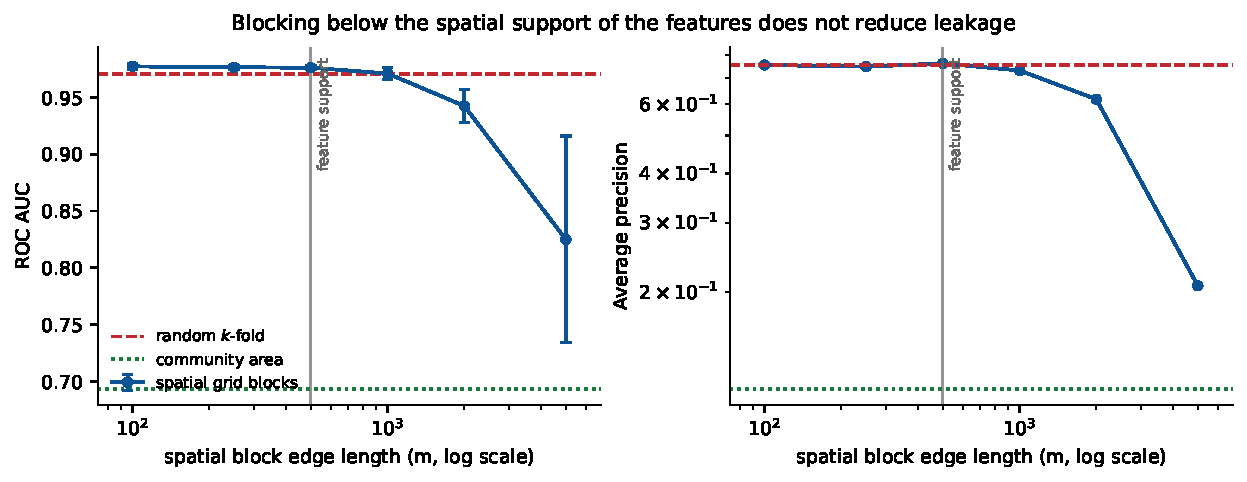
\includegraphics[width=\textwidth]{../outputs/figures/fig1_block_scale.pdf}
\caption{Performance against spatial block size. The curve is flat until blocks
exceed the $500$\,m spatial support of the features (grey line), then falls.
A practitioner selecting a block below that scale obtains an estimate
indistinguishable from random splits.}
\label{fig:scale}
\end{figure}

Table~\ref{tab:scale} and Figure~\ref{fig:scale} show performance is flat from
random splits through
$1$\,km blocks and falls only beyond $2$\,km. Since features summarise
neighbourhoods to $500$\,m, blocks at or below that scale cannot sever the
dependence they induce: information propagates as far as the blocks are wide.

The practical implication is a diagnostic rather than a fixed recommendation.
Sweeping block size and observing a flat curve indicates blocks are too small
relative to feature support; the curve's decline locates the scale at which
dependence is actually broken.

\subsection{Leakage scales with model capacity}

\begin{table}[t]
\centering
\begin{tabular}{lrrrrr}
\toprule
Model & Random AUC & Blocked AUC & $\Delta$ & Random AP & Blocked AP \\
\midrule
Logistic regression & $0.709$ & $0.696$ & $+0.013$ & $0.098$ & $0.098$ \\
$k$NN ($k=25$)      & $0.686$ & $0.616$ & $+0.070$ & $0.092$ & $0.072$ \\
Random forest       & $0.933$ & $0.686$ & $+0.247$ & $0.670$ & $0.086$ \\
Gradient boosting   & $0.970$ & $0.693$ & $+0.277$ & $0.756$ & $0.114$ \\
\bottomrule
\end{tabular}
\caption{Inflation by model family. Under blocked evaluation all families are
equivalent; under random splits they are not.}
\label{tab:models}
\end{table}

\begin{figure}[t]
\centering
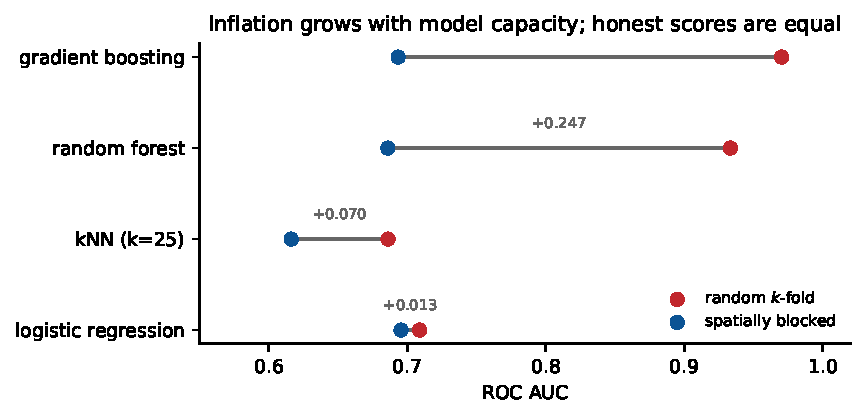
\includegraphics[width=0.78\textwidth]{../outputs/figures/fig2_model_families.pdf}
\caption{Paired random and blocked scores by model family. Honest scores
coincide; random-split scores do not, so the ranking is an artefact of the
partition.}
\label{fig:models}
\end{figure}

Table~\ref{tab:models} and Figure~\ref{fig:models} show inflation rising with
model flexibility. The
consequence extends beyond reporting. Under random cross-validation gradient
boosting appears to outperform logistic regression by $0.261$ AUC; under blocked
evaluation the gap is $-0.003$. Random splits therefore do not merely inflate a
figure, they invert a model-selection decision, and the inflation is largest
precisely for the model families practitioners most often prefer.

\subsection{Group aggregates dominate the leak}

\begin{table}[t]
\centering
\begin{tabular}{lrrrr}
\toprule
Feature family & $k$ & Random & Blocked & $\Delta$ \\
\midrule
Area aggregates (ward, community area) & 4 & $0.978$ & $0.657$ & $+0.321$ \\
Raw coordinates                        & 2 & $0.659$ & $0.595$ & $+0.064$ \\
Neighbourhood LOO ($50$--$500$\,m)     & 6 & $0.722$ & $0.687$ & $+0.034$ \\
Density counts                         & 3 & $0.694$ & $0.672$ & $+0.021$ \\
Building context                       & 2 & $0.508$ & $0.506$ & $+0.001$ \\
\bottomrule
\end{tabular}
\caption{Inflation by feature family, gradient boosting. Administrative
aggregates inflate an order of magnitude more than proximity features.}
\label{tab:ablation}
\end{table}

\begin{figure}[t]
\centering
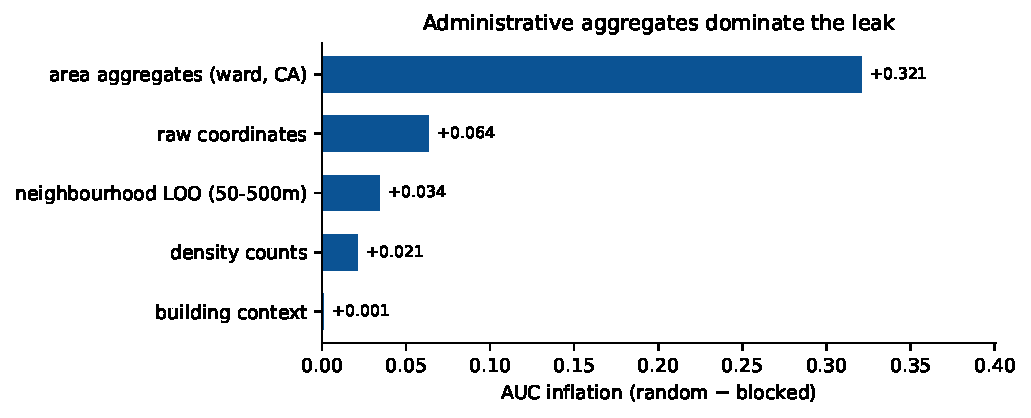
\includegraphics[width=0.78\textwidth]{../outputs/figures/fig3_feature_ablation.pdf}
\caption{AUC inflation by feature family. Administrative aggregates dominate;
proximity features contribute little.}
\label{fig:ablation}
\end{figure}

Table~\ref{tab:ablation} and Figure~\ref{fig:ablation} localise the leak to
administrative aggregates. Four
features alone reach AUC $0.978$ under random splits and $0.657$ under blocked
splits. Proximity features---the expected culprit---contribute little.

The mechanism is group identity rather than distance. A leave-one-out mean over a
ward is near-constant within that ward, so it serves as a ward identifier; under
a random split, training rows disclose the ward's label rate to test rows in the
same ward. Leave-one-out construction removes the focal observation but not the
remaining $n-1$, and with large groups this is negligible protection.

This reframes the requirement. What must align is not blocks with geography but
\emph{the evaluation partition with the grouping used to construct aggregate
features}. Where those groups are administrative units, spatial blocks of
arbitrary size do not satisfy it. Where the groups are not spatial at all---user,
merchant, session---the same failure arises with no spatial character, and the
same remedy applies.

\subsection{The substantive finding}

Under honest evaluation the urban result stands. Excess turnover concentrates at
individual addresses rather than districts. Leave-one-out neighbour turnover
exceeds the within-area permutation null by $+0.104$ tenants at $50$\,m
($p = 0.001$, null $+0.034 \pm 0.003$), $+0.068$ at $200$\,m and $+0.040$ at
$500$\,m, against a focal difference of $+1.99$ tenants. Neighbours of
high-turnover addresses are elevated by roughly $5\%$; the addresses themselves
by roughly $176\%$.

\begin{figure}[t]
\centering
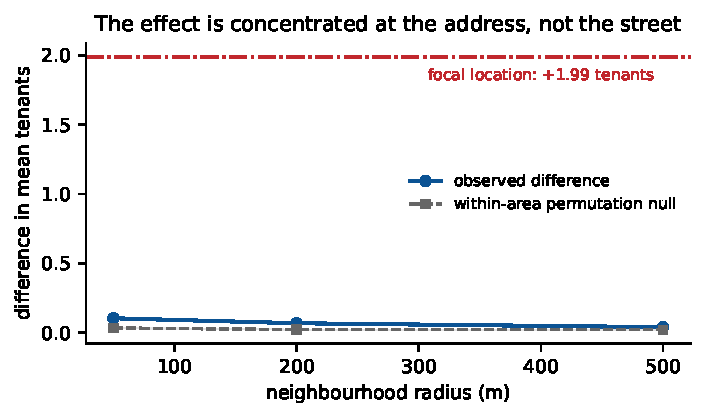
\includegraphics[width=\textwidth]{../outputs/figures/fig5_neighbour_decay.pdf}
\caption{Difference in mean tenant count between high-turnover locations and the
remainder, by neighbourhood radius, against a permutation null that shuffles
labels within community areas. The focal difference exceeds the neighbour
difference by an order of magnitude.}
\label{fig:decay}
\end{figure}

\begin{figure}[t]
\centering
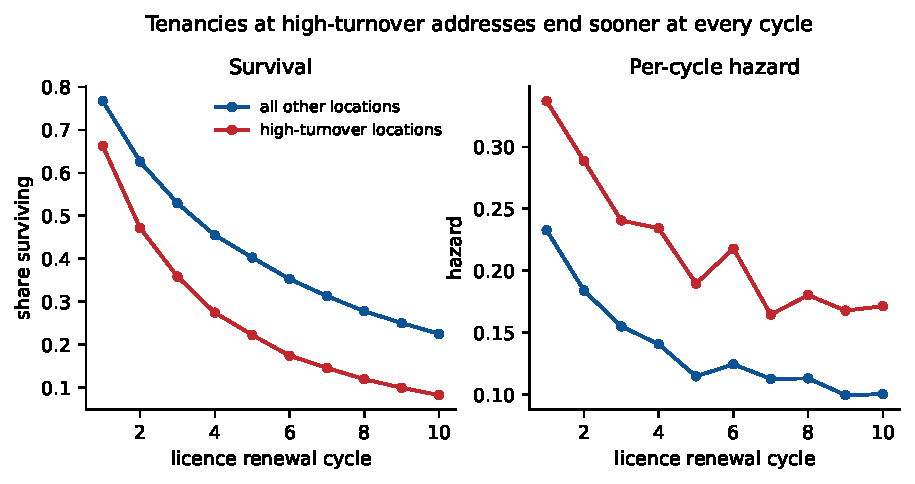
\includegraphics[width=\textwidth]{../outputs/figures/fig4_survival.pdf}
\caption{Discrete-time survival and per-cycle hazard over licence renewal
cycles. Renewal cycles are used in place of elapsed days because duration is
quantized to licence terms.}
\label{fig:survival}
\end{figure}

Discrete-time survival over renewal cycles (Figure~\ref{fig:survival}) shows
tenancies at these locations
ending faster at every stage: first-cycle hazard $0.337$ against $0.233$, and
survival to the eighth cycle of $0.119$ against $0.278$. The hazard ratio is
approximately constant across cycles, consistent with proportional hazards.

Context predicts the label only weakly (AUC $0.693$, AP $2.3\times$ base rate).
Most excess turnover is therefore not explained by observable surroundings.

\subsection{Sensitivity to the target definition}

\begin{table}[t]
\centering
\begin{tabular}{lrrr}
\toprule
 & Count & Rate & Excess \\
\midrule
Count ($\geq 4$ tenants)        & $1.000$ & $0.187$ & $0.193$ \\
Rate (tenants per decade, top $5\%$) & $0.187$ & $1.000$ & $0.632$ \\
Excess (model residual, top $5\%$)   & $0.193$ & $0.632$ & $1.000$ \\
\bottomrule
\end{tabular}
\caption{Jaccard overlap between the sets of locations flagged by three target
definitions.}
\label{tab:definitions}
\end{table}

Table~\ref{tab:definitions} reports agreement between the three definitions.
The exposure-adjusted definitions overlap substantially (Jaccard $0.632$), but
the unadjusted count-based definition overlaps both only weakly ($0.187$,
$0.193$). This is a genuine limitation and we state it plainly: which addresses
are called high-turnover depends materially on whether exposure and sector are
adjusted for, and a reader who prefers a raw-count definition would be studying
a substantially different set of locations.

We note that this sensitivity concerns the substantive finding rather than the
evaluation findings. The leakage results compare partitioning schemes holding
the target fixed, so they are unaffected by which definition is chosen; the
mechanism---group aggregates encoding group identity---depends on the feature
construction, not on the label.

\section{Recommendations}

\begin{enumerate}
\item \textbf{Partition by the grouping used for aggregate features.} If features
include group-level statistics, folds must respect those groups. This subsumes
spatial blocking when groups are geographic and applies unchanged when they are
not.
\item \textbf{Report a block-size sweep.} A flat performance curve across block
sizes indicates blocks below feature support. The curve costs little and makes
the claim auditable.
\item \textbf{Treat leave-one-out as insufficient.} It removes the focal
observation only. With large groups the remaining members carry essentially the
full signal.
\item \textbf{Compare model families under the final protocol.} Capacity-dependent
inflation means selection under random splits can invert under blocked splits.
\item \textbf{Report average precision with the base rate} for imbalanced targets.
\end{enumerate}

\section{Limitations}

Licence records proxy trading. A lapse may reflect administrative change rather
than closure; our succession merge is a conservative but imperfect correction,
and residual misclassification inflates apparent turnover.

Duration is interval-censored and quantized, which is why we use renewal cycles;
absolute tenure figures should not be read from this data.

Community area enters both the target definition and the partitioning, so
area-level comparisons are circular and excluded from substantive claims.

The single-city scope limits external validity of the urban finding. The
evaluation findings depend on the grouped structure of the features rather than
on Chicago specifically, but replication across cities remains future work.

Excess turnover is defined relative to a model, so the label inherits that
model's assumptions. Three alternative definitions are reported in the
supplement.

\section{Conclusion}

Spatially blocked cross-validation protects against optimistic evaluation only
when blocks are large relative to the spatial support of the features, and the
dominant leakage channel in this task is not proximity but group-aggregate
encoding over administrative units. Because that mechanism depends on grouping
rather than geography, it applies to any target-encoded grouped data. On our
task the difference between the default protocol and a correct one is AUC
$0.970$ versus $0.693$, and a reversal of model selection.

\section*{Reproducibility}

All inputs are public domain. Code, the download utility with row-count
verification, and the derived tenancy and location tables are released at
\url{https://github.com/naazzarov/storefront-turnover-leakage}. The pipeline is
deterministic given the seed reported in the repository.

\bibliographystyle{plainnat}
\begin{thebibliography}{99}

\bibitem[Dunne et al.(1988)]{dunne1988}
T.~Dunne, M.~J. Roberts, and L.~Samuelson.
\newblock Patterns of firm entry and exit in U.S. manufacturing industries.
\newblock \emph{RAND Journal of Economics}, 19(4):495--515, 1988.

\bibitem[Kapoor and Narayanan(2023)]{kapoor2023}
S.~Kapoor and A.~Narayanan.
\newblock Leakage and the reproducibility crisis in machine-learning-based
  science.
\newblock \emph{Patterns}, 4(9), 2023.

\bibitem[Kaufman et al.(2012)]{kaufman2012}
S.~Kaufman, S.~Rosset, C.~Perlich, and O.~Stitelman.
\newblock Leakage in data mining: Formulation, detection, and avoidance.
\newblock \emph{ACM TKDD}, 6(4):1--21, 2012.

\bibitem[Micci-Barreca(2001)]{micci2001}
D.~Micci-Barreca.
\newblock A preprocessing scheme for high-cardinality categorical attributes in
  classification and prediction problems.
\newblock \emph{ACM SIGKDD Explorations}, 3(1):27--32, 2001.

\bibitem[Ploton et al.(2020)]{ploton2020}
P.~Ploton et al.
\newblock Spatial validation reveals poor predictive performance of large-scale
  ecological mapping models.
\newblock \emph{Nature Communications}, 11:4540, 2020.

\bibitem[Prokhorenkova et al.(2018)]{prokhorenkova2018}
L.~Prokhorenkova, G.~Gusev, A.~Vorobev, A.~V. Dorogush, and A.~Gulin.
\newblock CatBoost: unbiased boosting with categorical features.
\newblock In \emph{NeurIPS}, 2018.

\bibitem[Roberts et al.(2017)]{roberts2017}
D.~R. Roberts et al.
\newblock Cross-validation strategies for data with temporal, spatial,
  hierarchical, or phylogenetic structure.
\newblock \emph{Ecography}, 40(8):913--929, 2017.

\bibitem[Valavi et al.(2019)]{valavi2019}
R.~Valavi, J.~Elith, J.~J. Lahoz-Monfort, and G.~Guillera-Arroita.
\newblock blockCV: An R package for generating spatially or environmentally
  separated folds.
\newblock \emph{Methods in Ecology and Evolution}, 10(2):225--232, 2019.

\end{thebibliography}

\end{document}
